% Created 2014-04-19 Sat 16:35
\documentclass{ctexart}
\usepackage[utf8]{inputenc}
\usepackage[T1]{fontenc}
\usepackage{fixltx2e}
\usepackage{graphicx}
\usepackage{longtable}
\usepackage{float}
\usepackage{wrapfig}
\usepackage{soul}
\usepackage{textcomp}
\usepackage{marvosym}
\usepackage{wasysym}
\usepackage{latexsym}
\usepackage{amssymb}
\usepackage{hyperref}
\usepackage{listings}
\usepackage{color}
\usepackage{xcolor}
\definecolor{background}{rgb}{0.9,0.9,0.9}
\tolerance=1000

\providecommand{\alert}[1]{\textbf{#1}}

\title{How to use sepDNA}
\author{GRC(扬眉剑)}
\date{\today}
\hypersetup{
  pdfkeywords={},
  pdfsubject={},
  pdfcreator={Emacs Org-mode version 7.9.3f}}

\begin{document}

\maketitle

\setcounter{tocdepth}{3}
\tableofcontents
\vspace*{1cm}
\section{环境配置}
\label{sec-1}

安装依赖的包:

\lstset{columns=flexible,backgroundcolor=\color{background},frame=trBL,frameround=fttt,breaklines=true,language=r}
\begin{lstlisting}
install.packages("RGtk2")
install.packages("gWidgetsRGtk2")
install.packages("RSQLite")
\end{lstlisting}

因为包RGtk2是依赖于GTK的,所以还要安装GTK。但是这里大家注意,不用自己去下载安装。
大家安装好RGtk2以后,然后用library(RGtk2)载入的时候,会提示让你安装Gtk。
你只需要选择安装就可以了。
这里还要注意一点,就是win64位系统的安装,大家如果用64位的R安装报错的话,那么安装
32位的R是一个明智的选择。(这里的报错包括后面编译sepDNA这个包)
\section{sepDNA的安装}
\label{sec-2}

这里提供给我们的是sepDNA\_1.0-6.tar.gz的文件。在windows系统下无法直接用R安装。
我们需要用到Rcmd。要使用Rcmd我们首先要把Rcmd命名所在的文件夹,添加到环境变量中。
Rcmd在R/bin/i386这个文件夹中。添加好以后,运行-cmd-Rcmd就会出现Rcmd命令的一些
选项。我们这里用到的是Rcmd的INSTALL功能,安装命令如下:

\lstset{columns=flexible,backgroundcolor=\color{background},frame=trBL,frameround=fttt,breaklines=true,language=Perl}
\begin{lstlisting}
Rcmd INSTALL D:\sepDNA_1.0-6.tar.gz
\end{lstlisting}
当然你可以选用-l选项来选择把包安装到不同的文件夹中。
\section{使用方法}
\label{sec-3}
\subsection{载入包}
\label{sec-3-1}

   \texttt{DEADLINE:} \textit{2014-04-19 Sat}

\lstset{columns=flexible,backgroundcolor=\color{background},frame=trBL,frameround=fttt,breaklines=true,language=r}
\begin{lstlisting}
library(sepDNA)
\end{lstlisting}
注意,sepDNA只能在R自带的RGui下使用,无法在Rstudio下面使用。
如果你在Rstudio下使用会得到以下报错信息:

\begin{verbatim}
Error in winMenuAddItem : function not supported in RStudio
\end{verbatim}
下面我们会看到我们载入包以后会在RGui中添加一个菜单项。但是这个添加却不能在RStudio中实现。

当我们加载以后,我们发现在R的菜单栏中出现了一个新的选项:sepDNA。
这个就是我们载入的包,sepDNA。我们后面就可以直接使用这个选项。

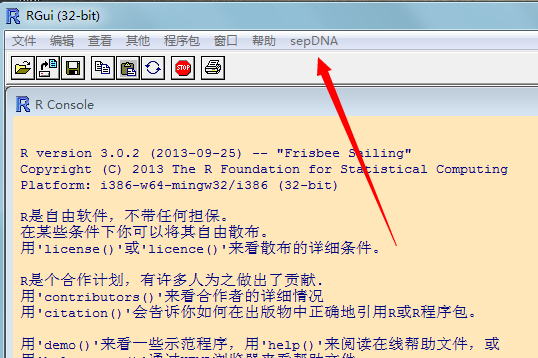
\includegraphics[width=.9\linewidth]{d:/Git/R/R_Course/R_Question_for_solve/sepDNA/sepDNA1.jpg}
\subsection{使用}
\label{sec-3-2}

我们点击sepDNA这个菜单以后,会出现四个选项。
\begin{itemize}
\item 系统设置(可以设置启动R自动加载)
\item 导入数据
\item 分析设置
\item 报告
\end{itemize}

我们着重来看后面三个
\subsubsection{数据导入}
\label{sec-3-2-1}

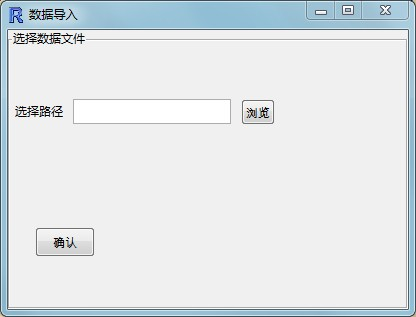
\includegraphics[width=.9\linewidth]{d:/Git/R/R_Course/R_Question_for_solve/sepDNA/sepDNA2.jpg}

sepDNA的包解压以后在inst/examples中会有一些实例文件用来分析。
我们导入数据以后会出现一个窗口让我们选择列名。我们依次选择:

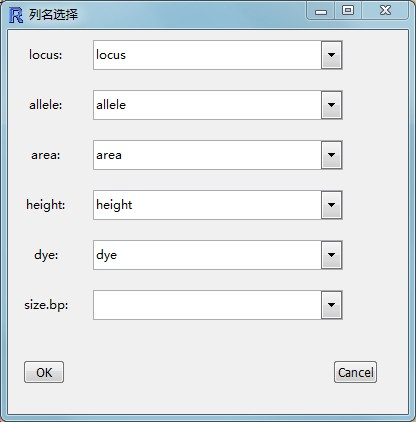
\includegraphics[width=.9 \linewidth]{d:/Git/R/R_Course/R_Question_for_solve/sepDNA/sepDNA3.jpg}

点击OK以后,数据成功导入。
\subsubsection{分析设置}
\label{sec-3-2-2}

我们打开分析设置的窗口,刚才导入的文件名已经在filename中。
点击连接数据,我们的R包会把基因座名称显示出来。
在分析选项中我们选择IDfiler,然后点击绘制图形。

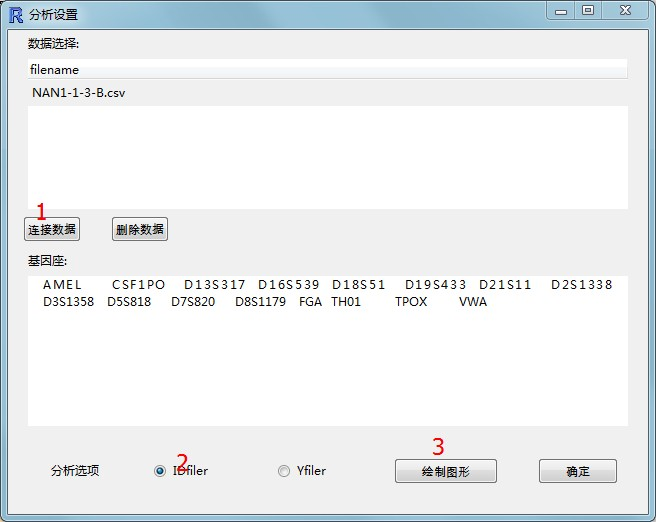
\includegraphics[width=.9\linewidth]{d:/Git/R/R_Course/R_Question_for_solve/sepDNA/sepDNA4.jpg}

然后就会按照数据进行画图分析。

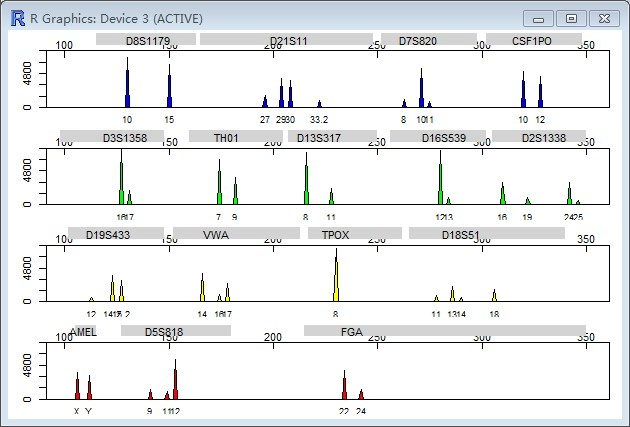
\includegraphics[width=.9\linewidth]{d:/Git/R/R_Course/R_Question_for_solve/sepDNA/sepDNA5.jpg}

\end{document}
